\let\negmedspace\undefined
\let\negthickspace\undefined
\documentclass[journal]{IEEEtran}
\usepackage[a5paper, margin=10mm, onecolumn]{geometry}
%\usepackage{lmodern} % Ensure lmodern is loaded for pdflatex
\usepackage{tfrupee} % Include tfrupee package
\setlength{\headheight}{1cm} % Set the height of the header box
\setlength{\headsep}{0mm}     % Set the distance between the header box and the top of the text
\usepackage{gvv-book}
\usepackage{gvv}
\usepackage{cite}
\usepackage{amsmath,amssymb,amsfonts,amsthm}
\usepackage{algorithmic}
\usepackage{graphicx}
\usepackage{textcomp}
\usepackage{xcolor}
\usepackage{txfonts}
\usepackage{listings}
\usepackage{enumitem}
\usepackage{mathtools}
\usepackage{gensymb}
\usepackage{comment}
\usepackage[breaklinks=true]{hyperref}
\usepackage{tkz-euclide} 
\usepackage{listings}
% \usepackage{gvv}                                        
\def\inputGnumericTable{}                                 
\usepackage[latin1]{inputenc}                                
\usepackage{color}                                            
\usepackage{array}                                            
\usepackage{longtable}                                       
\usepackage{calc}                                             
\usepackage{multirow}                                         
\usepackage{hhline}                                           
\usepackage{ifthen}                                           
\usepackage{lscape}
\begin{document}

\bibliographystyle{IEEEtran}
\vspace{3cm}
\parindent 0px

\title{6.6.11}
\author{EE24BTECH11050 - Pothuri Rahul}
% \maketitle
% \newpage
% \bigskip
{\let\newpage\relax\maketitle}

\renewcommand{\thefigure}{\theenumi}
\renewcommand{\thetable}{\theenumi}
\setlength{\intextsep}{10pt} % Space between text and floats


\numberwithin{equation}{enumi}
\numberwithin{figure}{enumi}
\renewcommand{\thetable}{\theenumi}

\textbf{Question :} \\ 
A window is in the form of a rectangle surmounted by a semicircular opening. The total perimeter of the window is 10 m. Find the dimensions of window to admit maximum light through the whole opening. \\
\solution \\
\textbf{Theoretical solution :} \\

\begin{figure}[!ht]
\centering
\resizebox{0.3\textwidth}{!}{%
\begin{circuitikz}
\tikzstyle{every node}=[font=\Large]
\draw [ line width=1.9pt](7.5,14.25) to[short] (7.5,9.5);
\draw [ line width=1.9pt](7.5,9.5) to[short] (13.5,9.5);
\draw [ line width=1.9pt](13.75,14.75) to[short] (13.75,9.5);
\draw [ line width=1.9pt](13.75,9.5) to[short] (13.25,9.5);
\draw [line width=1.9pt, short] (7.5,14.5) -- (7.5,13.5);
\draw [line width=1.9pt, short] (7.5,14.75) .. controls (8.75,18) and (12.5,17.75) .. (13.75,14.75);
\draw [line width=1.9pt, short] (7.5,14.75) -- (7.5,14.25);
\draw [line width=1.9pt, <->, >=Stealth] (14.75,14.5) -- (14.75,9.5);
\draw [line width=1.9pt, <->, >=Stealth] (10.75,14.75) -- (13.5,14.75);
\draw [line width=1.9pt, <->, >=Stealth] (7.5,8.75) -- (13.75,8.75);
\node [font=\Large] at (15.25,12) {a};
\node [font=\Large] at (12,15.25) {b};
\node [font=\Large] at (10.25,8.25) {2b};
\end{circuitikz}
}%
\end{figure}
From figuire, 
\begin{enumerate}
\item height and width of rectangle are a , 2b
\item radius of semi-circle is b
\end{enumerate}
from given data ,Perimeter = 10m 
\begin{align}
\brak{2\brak{a+2b}} + \brak{\pi b} = 10 \\
2a+b\brak{4+ \pi} = 10 \\
a = \frac{10 - b\brak{4+\pi}}{2} \label{1}
\end{align}
To get more light,We need maximum are for the window opening. \\
Let A be the area of the window opening, then \\
\begin{align}
A = 2ab + \frac{\pi b^2 }{2} \label{2}
\end{align}
By substituting \eqref{1} in \eqref{2}
\begin{align}
A = \brak{10 - b\brak{4+\pi}}b+\frac{\pi b^2}{2} \\ 
A = 10b - b^2 \brak{4+\pi} + \frac{\pi b^2}{2} \\ 
A = \frac{20b - b^2 \brak{8+2\pi} + \pi b^2}{2} \\
A = \frac{20b - b^2 \brak{\pi +8}}{2} \label{4}
\end{align}
Area A is the function of b,To get maximum $\frac{dA}{db} = 0$
By differentiating with respect to b,
\begin{align}
\frac{dA}{dt} = \frac{20 - 2 b \brak{\pi +8}}{2} = 0 \\
\implies 20 - 2b\brak{\pi +8} = 0 \\ 
\implies b = \frac{10}{\pi +8} \label{3}
\end{align}
by substituting \eqref{3} in \eqref{1} , 
\begin{align}
a = \frac{20}{\pi +8}
\end{align}
Dimensions of the rectangle are, 
\begin{align}
a = \frac{20}{\pi +8} \\ 
2b = \frac{20}{\pi +8}
\end{align}

\textbf{Using Gradient descent :-} \\
Gradient descent is a method used to find the minimum (or maximum ) of a given function. \\
We got Area as the function of b,So we can find the maximum area by Gradient ascent method (same as gradient descent) 
Area of the window opening in terms of b is given by 
\begin{align}
A = \frac{20b - b^2 \brak{\pi +8}}{2} 
\end{align} 
Gradient of the Area at any point b is given by 
\begin{align}
\frac{dA}{dt} = 10 - b \brak{\pi +8}
\end{align}
Let $\alpha$ be a learning rate,a small positive value that controls how much we move in the direction of the gradient. \\
Let us set the initial value of b, say $b_0$, to 0 and Area, say $A_0$ to 0. and update the b as ,
\begin{align}
b_{n+1} = b_n +\alpha \times \frac{dA}{db}
\end{align}
And calculate the value of A(Area) for the respective value of b using \eqref{4} \\
Now lets plot the values of A and b in the graph and we find the maximum A at a certain b in the plot.



\begin{figure}[htbp] % Positioning options: here, top, bottom, page
    \centering
    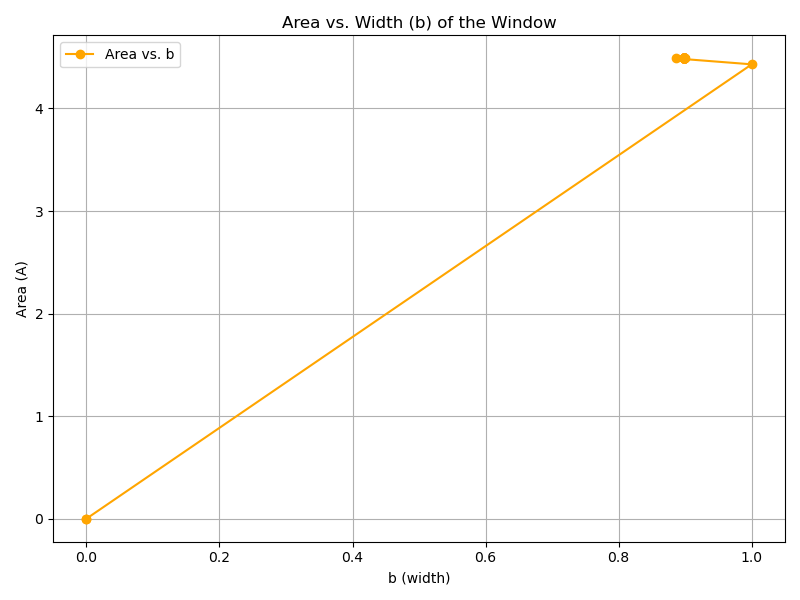
\includegraphics[width=\textwidth]{figs/plot.png} % Replace "filename" with your image file
    \caption{Plot}
\end{figure}





\end{document}
